
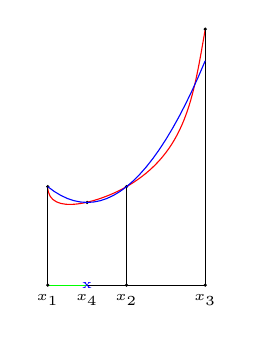
\begin{tikzpicture}
\draw (0,0) -- (2,0);
\draw [green](0,0) -- (0.5,0);
\draw[fill] (0,0) circle [radius=0.0125];
\node [below] at (0,0) {\tiny $x_1$};
\draw[fill] (2,0) circle [radius=0.0125];
\node [below] at (2,0) {\tiny $x_3$};
\draw[fill] (1,0) circle [radius=0.0125];
\node [below] at (1,0) {\tiny $x_2$};


\draw[red, domain=0:2] (0,1.25) [out=-90,in=-150] to (,1.25);
\draw[red, domain=0:2] (1,1.25) [out=-330,in=-100] to (2,3.25);



%\draw[blue, domain=0:2] plot (\x, {1+(\x-0.5)^2});
\draw (0,0) -- (0,1.25);
\draw[fill] (0,1.25) circle [radius=0.0125];
\draw (1,0) -- (1,1.25);
\draw[fill] (1,1.25) circle [radius=0.0125];
\draw (2,0) -- (2,3.25);
\draw[fill] (2,3.25) circle [radius=0.0125];
\node [blue] at (0.5,0){\tiny x};
\node [below] at (0.5,0){\tiny $x_4$};
\draw[fill] (.5,1.05) circle [radius=0.0125];
\draw[blue, domain=0:2] plot (\x, {1.25-0.8*\x+0.8*(\x)^2});


\end{tikzpicture}